\documentclass[conference]{IEEEtran}

\IEEEoverridecommandlockouts
% The preceding line is only needed to identify funding in the first footnote. If that is unneeded, please comment it out.


\usepackage{cite}
\usepackage{amsmath,amssymb,amsfonts}

\usepackage{graphicx,graphics,float}

\ifCLASSOPTIONcompsoc
    \usepackage[caption=false, font=normalsize, labelfont=sf, textfont=sf]{subfig}
\else
\usepackage[caption=false, font=footnotesize]{subfig}
\fi

\usepackage{textcomp}
\usepackage{xcolor}
\usepackage[utf8]{inputenc}
\usepackage[version-1-compatibility]{siunitx}
\usepackage{lettrine}
\usepackage{svg}
\usepackage[hidelinks]{hyperref}
\usepackage[noend]{algpseudocode}
\usepackage{algorithm}

\usepackage{makecell}

\hypersetup{
 colorlinks=false
}


\ifCLASSOPTIONcompsoc
    \usepackage[caption=false, font=normalsize, labelfont=sf, textfont=sf]{subfig}
\else
\usepackage[caption=false, font=footnotesize]{subfig}
\fi

\makeatletter
\@dblfptop 0pt
\makeatother

\def\BibTeX{{\rm B\kern-.05em{\sc i\kern-.025em b}\kern-.08em
    T\kern-.1667em\lower.7ex\hbox{E}\kern-.125emX}}
    
\begin{document}
\title{Item Recovery Problem\\\huge An ALNS-based Approach\\
}

\makeatletter
\newcommand{\linebreakand}{%
  \end{@IEEEauthorhalign}
  \hfill\mbox{}\par
  \mbox{}\hfill\begin{@IEEEauthorhalign}
}
\makeatother



\DeclareRobustCommand*{\IEEEautspihorrefmark}[1]{%
  \raisebox{0pt}[0pt][0pt]{\textsuperscript{\footnotesize #1}}%
}

\author{
\IEEEauthorblockN{
João Resende$^1$,
José Maravalhas-Silva$^2$
}
\IEEEauthorblockA{Doctoral Program in Electrical and Computer Engineering,\\ 
Faculty of Engineering, University of Porto,\\
Porto, Portugal\\
Email: up202003528@fe.up.pt$^1$, up202003505@fe.up.pt$^2$
}}


\maketitle

\begin{abstract}

This paper presents the implementation of the Adaptive Large Neighboorhood Search (ALNS) heuristic in solving the item recovery problem. This problem consists in optimizing the path taken by an Autonomous Underwater Vehicle (AUV) whose goal is to retrieve items from several different underwater sites.

\end{abstract}

\begin{IEEEkeywords}
Heuristics; Optimization; ALNS; AUV;
\end{IEEEkeywords}

\section{Introduction}

In the context of the course unit "Heuristics and Metaheuristics" from the  "Doctoral Program in Electrical and Computer Engineering" from the Faculty of Engineering, University of Porto (FEUP), this paper presents the implementation of an heuristic, known as the Adaptive Large Neighboorhood Search (ALNS) \cite{ALNS_book, ALNS_paper}, and its usage in solving an optimization problem inspired by currently ongoing projects at the Centre for Robotics and Autonomous Systems (CRAS) belonging to the Institute for Systems and Computer Engineering, Technology and Science (INESCTEC).

The problem comprises the optimization of the path taken by an AUV in such a way that the AUV is able to pick up and retrieve different items which are spread throughout multiple sites across the seabead. To the best of our knowledge, there is no literature that features this exact problem, thus we will name it the "item recovery problem".

\section{Problem Statement}

The following list defines the details and constrains of the item recovery problem:

\begin{itemize}
    \item[-] The AUV starts at a "base" site
    \item[-] There are multiple underwater sites that contain zero or more items that need to be "recovered" by the AUV
    \item[-] Every item has a given weight
    \item[-] The base site contains no items to be recovered
    \item[-] The AUV has a maximum carrying capacity
    \item[-] No item can exceed the maximum carrying capacity of the AUV by itself
    \item[-] When the AUV is at the base site, all items that it is currently carrying are unloaded (i.e. they are "recovered")
    \item[-] The AUV cannot unload items, except at the base site
    \item[-] A weighted graph is used to represent the sites and the distances between them
    \item[-] The goal is to recover all items while minimizing the total distance traveled
\end{itemize}

Figure \ref{fig:cave} illustrates a possible scenario of this problem, where an AUV is used to recover items from an underwater cave.

\begin{figure}[H]
  	  \centering
      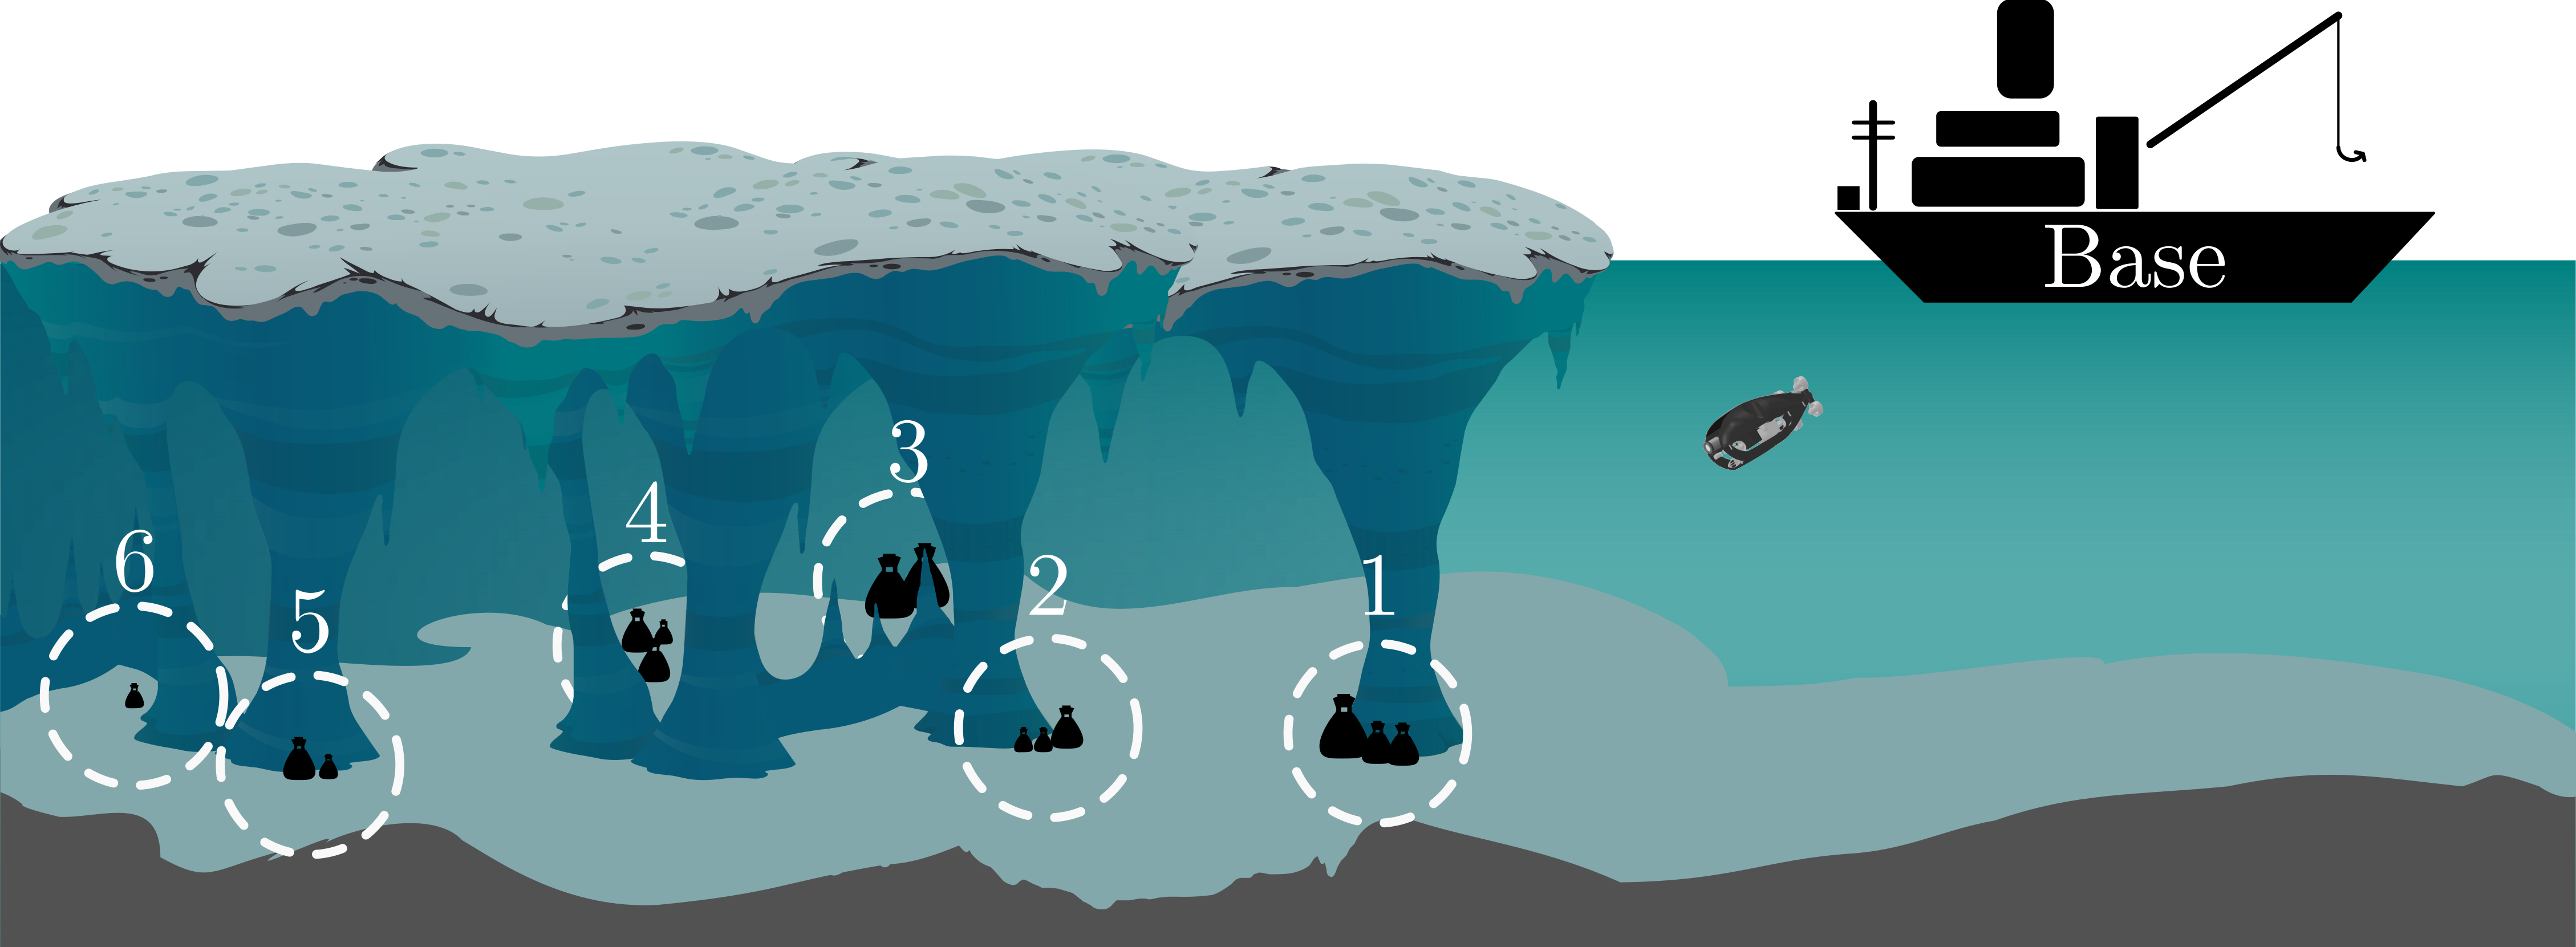
\includegraphics[width=\columnwidth]{./Figures/cave.png}
      \caption{Example of the item recovery problem.} 
      \label{fig:cave}
\end{figure}

The corresponding weighted graph is shown in Figure \ref{fig:graph}.

\begin{figure}[H]
  	  \centering
  	  \includesvg[width=\columnwidth]{./Figures/weighted_graph_example.svg}
      \caption{Weighted graph of the scenario shown in Figure \ref{fig:cave}. The items and their weights are shown to the right of each site.}
      \label{fig:graph}
\end{figure}

In Figure \ref{fig:graph}, the items and their weights are shown to the right of each site. For instance, site number 6 contains 2 items, one with a weight of 1 and another item with a weight of 2.

\section{Solution Representation}

The solution representation we used for this problem consists of a list of sites that the AUV visits. For each site, there is also a corresponding list of which items are picked.

A partial example of a solution for the scenario presented in Figures \ref{fig:cave} and \ref{fig:graph} is shown in Table \ref{tab:solution_representation}. This example assumes that items are indexed from top to bottom in Figure \ref{fig:graph}, and that the maximum carry weight is 4.

\begin{table}[ht]
\caption{Example of a solution}
\label{tab:solution_representation}
\resizebox{\columnwidth}{!}{%
\begin{tabular}{|c|c|c|c|c|c|c|c|c|c|c|}
\hline
Path & Base & 1 & 2 & 1 & Base & 3 & 4 & 3 & Base & ... \\ \hline
\begin{tabular}[c]{@{}c@{}}Items\\ Picked\end{tabular} & {[\,]} & {[0]} & {[0]} & {[\,]} & {[\,]} & {[\,]} & {[0,1]} & {[\,]} & {[\,]} & ... \\ \hline
\end{tabular}
}
\end{table}

As per the constrains of the problem, the AUV starts at the base site, and then moves to site 1 and picks up item 0, which has a weight of 2, as shown in Figure \ref{fig:graph}. It then moves to site 2 to pick up item 2, which also has a weight of 2. Having a full cargo, the AUV can no longer pick up any more items, and goes through site 1 to reach the base site and complete the retrieval. Looking at the graph and its weights, one obvious optimization to apply to this part of the solution would be to go directly to the base site from site 2.


\section{Optimization Technique}

The proposed optimization technique is based on the Adaptive Large Neighborhood Search (ALNS) heuristic. In this section, we present both the generic implementation of the ALNS heuristic as well as our own procedures that are then fed to the ALNS-based optimization algorithm.

\subsection{ALNS Heuristic}

The first appearance of the ALNS heuristic was proposed in \cite{ALNS_paper} in order to solve a pickup and delivery problem with time windows. This heuristic is an extension of the Large Neighborhood Search (LNS) heuristic \cite{LNS_paper}. Whereas the original LNS heuristic repeatedly applies a single destruction method and a single repair method, the ALNS heuristic uses pools of destruction and repair methods and dynamically updates the methods used in each iteration according to their past successes and failures.

The means by which destruction and repair methods are selected is via weights that define their probability of being chosen for the current iteration of the algorithm. The weights are then dynamically adjusted at the end of the iteration\cite{ALNS_book}.

\begin{algorithm}[htp]
\caption{Adaptive Large Neighborhood Search \cite{ALNS_book}.}
\label{alg:alns_algorithm}
\begin{algorithmic}[1]
\State \textbf{input} a feasible solution $x$
\State $x^b = x$; $\rho^- = (1,...,1)$; $\rho^+ = (1,...,1)$
\Repeat
    \State Select a destruction method $d \in \Omega^-$ according to $\rho^-$
    \State Select a repair method $r \in \Omega^+$ according to $\rho^+$
    \State $x^t = r(d(x))$
    \If{ accept($x^t$,$x$) }
        \State $x=x^t$
    \EndIf
    \If{ $cost(x^t) < cost(x^b)$ }
        \State $x^b = x^t$
    \EndIf
    \State Update $\rho^-$ and $\rho^+$;
\Until{stop criterion is met}
\State \Return $x^b$
\end{algorithmic}
\end{algorithm}

\pagebreak
Algorithm \ref{alg:alns_algorithm} demonstrates the high-level implementation of the ALNS heuristic. In this algorithm, $x^t$ is the solution of the current iteration, $x^b$ is the best known solution, and $\Omega^-$ and $\Omega^+$ are the pools (i.e. the sets) of destroy and repair methods, respectively. Destruction and repair methods have associated weights $\rho^-$ (for destruction methods) and $\rho^+$ (for repair methods), such that $\rho^- \in \mathbb{R}^{|\Omega^-|}$ and $\rho^+ \in \mathbb{R}^{|\Omega^+|}$.

In order to choose the methods in lines 4 and 5, a roulette wheel selection method is used. The probability $\varphi^\pm_{j}$ of selecting any given destruction ($\varphi^-_{j}$) or repair ($\varphi^+_{j}$) method $j$ belonging to $\Omega^\pm$ is given by:

\begin{equation}\label{eq:line4_weight_prob}
\varphi^\pm_{j} = \frac{\rho^\pm_{j}}{\sum_{i=1}^{|\Omega^\pm|}\rho^\pm_{i}}
\end{equation}

For the dynamic update of the weights at the end of each iteration (line 13), a score $\Psi$ is computed according to the following equation:

\begin{equation*}\label{eq:score_formula}
\Psi = max \begin{cases} 
\omega_{1}, \text{if the new solution is a new global best.} \\
\omega_{2}, \text{if the new solution is better than the current.} \\
\omega_{3}, \text{if the new solution is accepted.} \\
\omega_{4}, \text{if the new solution is rejected.} \\
\end{cases}
\end{equation*}

where $\omega_{1}$, $\omega_{2}$, $\omega_{3}$ and $\omega_{4}$ are non-negative constants.

For both the destruction and repair methods used in the current iteration, their respective weights are updated as follows:

\begin{equation}\label{eq:weight_update}
\rho^\pm_{i} = \lambda \rho^\pm_{i} + (1 - \lambda)\Psi
\end{equation}

where $\lambda \in [0,1]$ is the decay parameter that controls how much influence past scores have in relation to the current score $\Psi$. Notice how equation \ref{eq:weight_update} effectively resembles the backward Euler discretization of a first order low-pass filter.

\subsection{Destruction Methods}

This subsection contains all the implementations and illustrative examples of the destruction methods we used to solve the item recovery problem.

\subsubsection{Random Position Removal}

This destruction method removes anywhere between 10\% and 60\% of all positions along the solution's path.

Algorithm \ref{alg:remove_rand_pos} demonstrates exactly how this is implemented. Note how the algorithm includes and additional check to ensure that the solution is never empty.

An example of random positions being removed from a solution is shown in Figure \ref{fig:remove_rand_pos}.

\begin{figure}[ht]
  	  \centering
  	  \includesvg[width=\columnwidth]{./Figures/destruction/remove_rand_pos.svg}
      \caption{Example of random positions being removed from a solution.}
      \label{fig:remove_rand_pos}
\end{figure}

\begin{algorithm}[h]
\caption{Random Position Removal}
\label{alg:remove_rand_pos}
\begin{algorithmic}[1]
\State \textbf{input} solution $x$
\State N = random(0.1, 0.6) * size($x$)
\State N = max(1, floor(N))
\While{N != 0 and size($x$) $>$ 1}
    \State Remove a random position from $x$
    \State N = N - 1
\EndWhile
\State \textbf{return} solution $x$
\end{algorithmic}
\end{algorithm}

\subsubsection{Random Position Swap}

This destruction method randomly swaps (at most) 20\% of all positions along the solution's path.  Picked up items are also swapped along with their respective positions. 

Algorithm \ref{alg:swap_rand_pos} demonstrates the implementation of this destruction method, and an example is shown in Figure \ref{fig:swap_rand_pos}.

\begin{figure}[h]
  	  \centering
      \includesvg[width=\columnwidth]{./Figures/destruction/swap_rand_pos.svg}
      \caption{Example of random positions being swapped in a solution.}
      \label{fig:swap_rand_pos}
\end{figure}

\begin{algorithm}[h]
\caption{Random Positions Swap}
\label{alg:swap_rand_pos}
\begin{algorithmic}[1]
\State \textbf{input} solution $x$
\State N = 0.2 * size($x$)
\State N = max(1, floor(N))
\While{N != 0}
\State Swap two random positions in solution $x$
\State N = N - 1
\EndWhile
\State \textbf{return} solution $x$
\end{algorithmic}
\end{algorithm}


\subsubsection{Random Subpath Removal}

This destruction method randomly removes between 10\% and 60\% of all subpaths. A subpath is any part of a solution contained between two visits to the base site. It should be noted that when removing a subpath, a visit to the base site must be left in its place in order not to leave other subpaths incomplete.

Algorithm \ref{alg:remove_rand_sps} demonstrates the implementation of this destruction method, and an example is shown in Figure \ref{fig:remove_rand_sps}.

\begin{figure}[ht]
  	  \centering
  	  \includesvg[width=\columnwidth]{./Figures/destruction/remove_rand_sps.svg}
      \caption{Example of random subpaths being removed from a solution}
      \label{fig:remove_rand_sps}
\end{figure}

\begin{algorithm}[h]
\caption{Random Subpaths Removal}
\label{alg:remove_rand_sps}
\begin{algorithmic}[1]
\State \textbf{input} solution $x$
\State N = random(0.1, 0.6) * number\_subpaths($x$)
\State N = max(1, floor(N))
\While{N != 0 and number\_subpaths($x$) $>$ 1}
\State Remove a random subpath from solution $x$
\State N = N - 1
\EndWhile
\State \textbf{return} solution $x$
\end{algorithmic}
\end{algorithm}

\subsubsection{Remove Worst Subpaths}

In this destruction operator, all subpaths are ranked according to a "score" value. Each subpath's score $S_i$ is based on how much item weight is retrieved during the subpath and how much cost does the subpath add to the overall solution:

\begin{equation}\label{eq:remove_worst_sps}
S_i = \frac{\text{total item weight retrieved in subpath } i}{\text{cost of subpath }i}
\end{equation}

After ranking all subpaths, between 10\% and 60\% of the worst scoring subpaths are removed. Algorithm \ref{alg:remove_worst_sps} demonstrates the implementation of this destruction method, and an example is shown in Figure \ref{fig:remove_worst_sps}. The costs and item weights are taken from the scenario shown in Figure \ref{fig:graph}.

\begin{figure}[h]
  	  \centering
  	  \includesvg[width=\columnwidth]{./Figures/destruction/remove_worst_sps.svg}
      \caption{Example of the worst subpaths being removed from a solution}
      \label{fig:remove_worst_sps}
\end{figure}

\begin{algorithm}[h]
\caption{Worst Subpaths Removal}
\label{alg:remove_worst_sps}
\begin{algorithmic}[1]
\State \textbf{input} solution $x$
\For{each subpath $i$ in solution $x$}
\State Compute $S_i$
\EndFor
\State N = random(0.1, 0.6) * number\_subpaths($x$)
\State N = max(1, floor(N))
\While{N != 0 and number\_subpaths($x$) $>$ 1}
\State Remove subpath $i$ with lowest $S_i$ from solution $x$
\State N = N - 1
\EndWhile
\State \textbf{return} solution $x$
\end{algorithmic}
\end{algorithm}


\subsection{Repair Method}

Since repairing a solution for the item recovery problem is a particularly involved process, only a single repair method has been developed. This method is divided into multiple steps that progressively repair different aspects of the solution.

\subsubsection{First Step}

A valid solution must always begin at the base, and end at the base. To ensure this, the first step checks if the solution starts at the base, and merely inserts it at the begin of the solution's path if it is not present.

Similarly, if the solution does not end at the base, the solution is truncated - i.e. the last position is removed from the solution until the last position of the path is the base.

Algorithm \ref{alg:greedy_repair_step_1} demonstrates how this repair step is implemented.

\begin{algorithm}[h!]
\caption{First Step of the Repair Method}
\label{alg:greedy_repair_step_1}
\begin{algorithmic}[1]
\State \textbf{input} solution $x$
\If{Solution does not start at the base}
\State Insert "Base" at the beginning of solution $x$
\EndIf
\While{Solution does not end at the base}
\State Remove last position from solution $x$
\EndWhile
\end{algorithmic}
\end{algorithm}

\subsubsection{Second Step}

A valid solution must never have "invalid" moves (i.e. edges on the weighted graph that do not exist) along the path, nor should it have consecutive visits to the same site as these do not add any useful information.

The second step of the repair method traverses the path of the solution and inserts the shortest path between two sites whenever direct movement between said sites is impossible. The shortest path is computed using Dijkstra's algorithm.

Additionally, this step also merges any consecutive visits to the same site that may occur along the solution, along with their lists of picked up items.

Algorithm \ref{alg:greedy_repair_step_2} demonstrates how this step is implemented.

\begin{algorithm}[h!]
\caption{Second Step of the Repair Method}
\label{alg:greedy_repair_step_2}
\begin{algorithmic}[1]
\State \textbf{input} solution $x$
\State $i$ = $0$
\While{$i$ $<$ size($x$)$- 1$}
\If{site at $x[i]$ == site at $x[i+1]$}
\State Add picked items from $x[i+1]$ to $x[i]$
\State Delete $x[i+1]$
\ElsIf{no connection between $x[i]$ and $x[i+1]$}
\State $repair\_path$ = Dijkstra(Site at $x[i]$, Site at $x[i+1]$)
\State Insert $repair\_path$ between $x[i]$ and $x[i+1]$
\Else
\State $i$ = $i + 1$
\EndIf
\EndWhile
\end{algorithmic}
\end{algorithm}

It should be noted that in Algorithm \ref{alg:greedy_repair_step_2}, no items are picked up along $repair\_path$.

\subsubsection{Third Step}

A valid solution must never exceed the maximum carry weight. Thus, the third step of the repair method checks all subpaths within the solution, and, if necessary, randomly removes picked up items along each subpath that exceeds the carry weight until it is no longer exceeded.

Algorithm \ref{alg:greedy_repair_step_3} demonstrates how this repair step is implemented.


\begin{algorithm}[h!]
\caption{Third Step of the Repair Method}
\label{alg:greedy_repair_step_3}
\begin{algorithmic}[1]
\State \textbf{input} solution $x$
\For{\textbf{each} $subpath$ in solution $x$}
\While{$max\_carry\_weight$ in $subpath$ is exceeded}
\State \parbox[t]{\dimexpr\textwidth-\leftmargin-\labelsep-\labelwidth}{Remove a random item from a random position\\in $subpath$\strut}
\EndWhile
\EndFor
\end{algorithmic}
\end{algorithm}


\subsubsection{Fourth Step}

After the third step, the solution will likely be missing multiple items that still need to be recovered. 

The fourth step of the repair procedure attempts to perform zero-cost insertions of the missing items in the current solution.

Algorithm \ref{alg:greedy_repair_step_4} demonstrates how the zero-cost insertions are performed.

\begin{algorithm}[h!]
\caption{Fourth Step of the Repair Method}
\label{alg:greedy_repair_step_4}
\begin{algorithmic}[1]
\State \textbf{input} solution $x$
\For{\textbf{each} item $i$ at site $j$ that has not been recovered}
\State $candidates$ = all indexes of $x$ where site $j$ is visited
\While{item $i$ at site $j$ has not been recovered\\\ \ \ \ \ \ \ \ \ \ \ \ \textbf{and} size($candidates$) != $0$}
\State $candidate$ = select random value from $candidates$
\State $subpath$ = subpath where $candidate$ is contained
\If{total item weight recovered in $subpath$ + weight\\\ \ \ \ \ \ \ \ \ \ \ \,of item $i$ at site $j$ $<=$ $max\_carry\_weight$}
\State Insert item $i$ (from site $j$) in $x[candidate]$
\Else
\State Remove $candidate$ from $candidates$
\EndIf
\EndWhile
\EndFor
\end{algorithmic}
\end{algorithm}


\subsubsection{Fifth Step}

After the previous step, any items that have not yet been recovered can not be inserted at zero-cost in the current solution. Therefore, this step now appends new subpaths to the solution to pick up the remaining items.

Algorithm \ref{alg:greedy_repair_step_5} demonstrates how this repair step is implemented.

\begin{algorithm}[h!]
\caption{Fifth Step of the Repair Method}
\label{alg:greedy_repair_step_5}
\begin{algorithmic}[1]
\State \textbf{input} solution $x$
\While{not all items have been recovered}
\State $item$ = random item that has not been recovered
\State $site$ = site where $item$ is located
\State $subpath$ = Dijkstra(Base, $site$) + Dijkstra($site$, Base)
\State \parbox[t]{\dimexpr\textwidth-\leftmargin-\labelsep-\labelwidth}{Append $subpath$ to solution $x$, ensuring that $item$\\is picked up along the way\strut}
\EndWhile
\end{algorithmic}
\end{algorithm}

It should be noted that in Algorithm \ref{alg:greedy_repair_step_5}, line 5's implementation should not result in consecutive visits to the same site.

\subsubsection{Sixth Step}

Technically, the sixth step is not necessary as the solution is guaranteed to be valid after the previous step. However, since the solution might contain subpaths where items are not picked up, removing them can help the intensification of the search algorithm, at the expense of diversification. This is not a problem, since the ALNS heuristic is already extremely diversified, as the destruction methods remove significant portions of the solution.

Algorithm \ref{alg:greedy_repair_step_6} demonstrates how the final post-processing step is implemented.

\begin{algorithm}[h!]
\caption{Sixth Step of the Repair Method}
\label{alg:greedy_repair_step_6}
\begin{algorithmic}[1]
\State \textbf{input} solution $x$
\For{\textbf{each} $subpath$ in $x$}
\If{no items are picked along $subpath$}
\State Remove $subpath$ from solution $x$
\EndIf
\EndFor
\end{algorithmic}
\end{algorithm}

\subsection{Initial Solution}

To generate the initial solution necessary for the ALNS heuristic, the repair method is called for a solution that has a single position, which is the base. This will make it such that all steps from 1 to 4 will fail to do anything, and step 5 will then generate a subpath for each item to be recovered.

\subsection{Acceptance Criterion}

For the acceptance criterion, a simulated annealing technique with linear temperature cooldown was used.

\section{Results}

\subsection{Dataset}

Since there are no pre-existing datasets of instances of the item recovery problem, we've created our own dataset. Some general information about the dataset is shown in Table \ref{tab:instances}.

This dataset contains instances with anywhere from 40 to 100 sites. 

In each instance, the carry weight $C$ is randomly selected in the range $[2,10]$. 

The maximum number of items per site ($M_i$) was randomized between $[5, 10]$ for each instance. Then, when generating said instance, the actual number of items in each site is randomly selected between $[0, M_i]$. 

All item weights are also randomly selected. In each instance, these weights have a minimum of 1, and a randomly chosen maximum in the range $[2, C]$.

For the connections between sites, all sites are connected to at least 1 other site. The actual number of connection ranges between $[1, M_c]$, where $M_c$ is randomly selected between $[2, 5]$ for each instance.

It should be noted that the dataset used does not necessarily represent real-world scenarios. In our dataset's instances, while the connections between sites are relatively sparse, they are still completely random. In real-world scenarios, these connections would, most likely, not be random, but rather possess some structure to them.

\begin{table}[h!]
\caption{General Information of the Dataset Used}
\label{tab:instances}
\centering
\resizebox{0.8\columnwidth}{!}{%
\begin{tabular}{|c|c|c|c|c|}
\hline
Instance & Sites & \makecell{Sites With\\Items} & \makecell{Cargo\\Size} & \makecell{Graph\\Edges} \\ \hline
1 & 40 & 36 & 2 & 101 \\ \hline
2 & 45 & 39 & 9 & 112 \\ \hline
3 & 50 & 44 & 4 & 66 \\ \hline
4 & 55 & 47 & 7 & 111 \\ \hline
5 & 60 & 49 & 3 & 140 \\ \hline
6 & 65 & 61 & 6 & 98 \\ \hline
7 & 70 & 63 & 3 & 169 \\ \hline
8 & 75 & 62 & 5 & 193 \\ \hline
9 & 80 & 68 & 4 & 185 \\ \hline
10 & 85 & 72 & 9 & 170 \\ \hline
11 & 90 & 72 & 9 & 228 \\ \hline
12 & 95 & 86 & 9 & 236 \\ \hline
13 & 100 & 91 & 10 & 156 \\ \hline
\end{tabular}
}
\end{table}

\subsection{Optimization Results}

Table \ref{tab:optimization_results} contains the optimization results for all instances of our dataset after 200 iterations of the search algorithm. 

The initial temperature of the simulated annealing acceptance criterion was set to 100, with each iteration of the search algorithm reducing this value by 5, down to a minimum of 5.

As an example, Figures \ref{fig:inst1} and \ref{fig:inst1_methods} contain information on the best and accepted costs per iteration, as well as diagnostics for all methods, for instance 1. We've found that other instances also follows similar trends.

\begin{figure}[h!]
  	  \centering
  	  \includesvg[width=\columnwidth]{./Figures/instance_1.svg}
      \caption{Best and accepted Costs at each iteration - Instance 1}
      \label{fig:inst1}
\end{figure}

\begin{figure}[h!]
  	  \centering
  	  \includesvg[width=\columnwidth]{./Figures/instance_1_methods.svg}
      \caption{Method diagnostics - Instance 1}
      \label{fig:inst1_methods}
\end{figure}

\pagebreak

\begin{table}[h!]
\caption{Optimization Results}
\label{tab:optimization_results}
\centering
\resizebox{0.8\columnwidth}{!}{%
\begin{tabular}{|c|c|c|c|}
\hline
Instance & Time Taken & Initial Cost & Best Cost \\ \hline
1 &  28 min & 5258 & 3421 \\ \hline
2 &  1 h & 5724 & 2856 \\ \hline
3 &  1.3 h & 9254 & 6046 \\ \hline
4 &  2.1 h & 13280 & 8072 \\ \hline
5 &  1.6 h & 8098 & 3797 \\ \hline
6 &  9.7 h & 16120 & 9928 \\ \hline
7 &  6.7 h & 6028 & 2818 \\ \hline
8 &  5.5 h & 11614 & 7354 \\ \hline
9 &  5.5 h  & 8474 & 4040 \\ \hline
10 &  9.4 h & 7966 & 5018 \\ \hline
11 &  2.2 h & 7560 & 3125 \\ \hline
12 &  10.5 h & 20932 & 6192 \\ \hline
13 & 51.6 h & 35946 & 23444 \\ \hline
\end{tabular}
}
\end{table}



\section{Conclusions}

In this work we presented an optimization problem inspired by real underwater robotics projects and employed the ALNS heuristic to solve it. 

The four destruction methods and the repair method implemented allowed for significant improvements over the initial solutions, but without knowing the optimal cost for each instance (or at least knowing some lower bound for it), it is difficult to ascertain whether or not our results are satisfactory.

Regarding the destruction methods used, it was clear from the method diagnostics from multiple instances that the "random position swap" method was not very effective. In most instances, it never resulted in any improvement, only occasionally being accepted. If the acceptance criteria was a typical hill climbing criterion, then this method would have been useless every single time.

The ineffectiveness of the "random position swap" is likely related to how it interacts with the repair method. Whenever a swap occurs, the solution will either remain valid, or it will have impossible connections between sites, depending on the sites being swapped and their neighbors. Consequently, the repair method may have to insert repair paths between the swapped sites and their neighbors, which will increase the overall's solution cost. If the swaps end up exceeding the carry weight on some supaths, some items will then need to be removed, which could lead to the repair method having to append additional subpaths to recover the remaining items that cannot be inserted back into the solution at zero-cost.

As for the time taken to process 200 steps of the search algorithm, we believe significant performance gains could be achieved by carefully optimizing our source code. While the number of iterations was kept to a small value to reduce the time necessary to run the algorithm, it's clear that many more iterations were needed to find better solutions, particularly on the instances with more sites.

Another possible future improvement to implement would be to dynamically update the degree of destruction - i.e. the percentage of the solution to be destroyed. This would likely entail the modification of the ALNS heuristic itself to include such a parameter, and research would need to be carried out to determine if this parameter should be specific to each destruction method, or shared between all destruction methods.

All source code and instances used can be accessed via our GitHub repository\cite{github}.

\bibliographystyle{IEEEtran}
\bibliography{references}
\end{document}
